\section{Technology Assessment}
\label{sec:technology}


Introduce in (sufficient) depth the key concepts and architecture of the chosen software technology. As part if this, you may consider using a running example to introduce the technology.

This part and other parts of the report probably needs to refer to
figures. Figure~\ref{fig:framework} from \cite{brown:96} just
illustrates how figure can be included in the report.

\begin{figure}[thb]
	\centering
	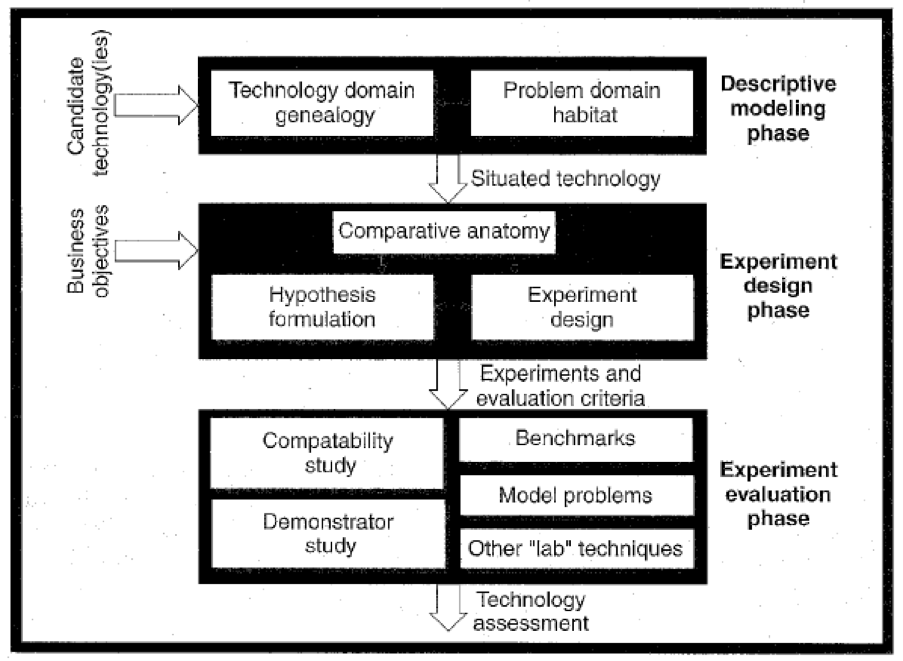
\includegraphics[scale=0.5]{figs/framework.png}
	\caption{Software technology evaluation framework.}
	\label{fig:framework}
\end{figure}

\subsection{Descriptive Modeling}

write where the technology comes from, its history, its context and what problem it solves.
Consider drawing a graph like in \cite{brown:96}.
\\
Neo4j originates from 2000 when Emil Eifrem and his team at Neo Technology began developing a database solution to handle complex, interconnected data more efficiently than traditional relational databases could. The first version of Neo4j was released in 2007 as an open-source graph database. It quickly gained traction where developers and enterprises needed flexible data models. Neo4j is now one of the most widely used graph databases.

relational databases (SQL) are efficient for structured data, Neo4j was created as an answer to the problem where relational databases would struggle with highly connected data. 

So in the late 2000s Neo4j emerged with the NoSQL movemevent where organizations needed more flexible scalable and schema free databases. Other NoSQL types are key-value stores, document stores and column family stores all solving specific problems, graph databases like Neo4j targets relationship-heavy data.

The problem Neo4j solve is where relationships are as important as the data itself. This is ideal for social networks which we could eventually want to use, or recommendation systems where we were thinking you could recommend relevant polls to users.

\subsection{Experiment Design}

Write you hypotheses about what benefits the technology bring and how you can support or reject them via experiments.
\\

We believe that in this case where we are creating a Poll App, our hypotheses is that using Neo4j as our cache will be beneficial for us as we are storing things which makes sense to put into a graph database. We also believe it will be easier to use then a key-value store for example because it is easier as developers to visualize the data and see what is happening behind the scenes. In this example we are doing here it will most likely not be quicker then a traditional NoSql database as for example Redis which is a key-value store. Since this is a relatively small app and we dont expect to high traffic we dont believe that efficiency is the most important part. We believe Neo4j can be beneficial if we were to choose to add additional functionality like for example adding friends and getting recommended polls based on earlier polls you have voted on, which would be a logical next step. We also believe having the cypher query language will make it easier for us to find our data, then using traditional look up. To support our hypotheses we will try to benchmark the quickness of neo4j versus redis which we already have implemented. Comparing these will give us an idea of the difference. Then we will look into the ease of use for both of these and the visualization ability. Then we can look at the tradeoff from both and see if neo4j is a viable option.

\subsection{Experiment Evaluation}

Write about the results of your experiments, either via personal experience reports, quantitative benchmarks, a demostrator case study or a combination of multiple approaches.


For some reports you may have to include a table with experimental
results are other kinds of tables that for instance compares
technologies. Table~\ref{tab:results} gives an example of how to create a table.

\begin{table}[bth]
	\centering
	\begin{tabular}{llrrrrrr}
		Config & Property & States & Edges & Peak & E-Time & C-Time & T-Time
		\\ \hline \hline
		22-2 & A   &    7,944  &   22,419  &  6.6  \%  &  7 ms & 42.9\% &  485.7\% \\
		22-2 & A   &    7,944  &   22,419  &  6.6  \%  &  7 ms & 42.9\% &  471.4\% \\
		30-2 & B   &   14,672  &   41,611  &  4.9  \%  & 14 ms & 42.9\% &  464.3\% \\
		30-2 & C   &   14,672  &   41,611  &  4.9  \%  & 15 ms & 40.0\% &  420.0\% \\ \hline
		10-3 & D   &   24,052  &   98,671  & 19.8  \%  & 35 ms & 31.4\% &  285.7\% \\
		10-3 & E   &   24,052  &   98,671  & 19.8  \%  & 35 ms & 34.3\% &  308.6\% \\
		\hline \hline
	\end{tabular}
	\caption{Selected experimental results on the communication protocol example.}
	\label{tab:results}
\end{table}
